\vspace*{-1mm}

1. present brifly the parameters
2. injected rf noise
3. MD emittance growth overview. 
    - average from IN and OUT. As mentioned in CH4. vs time and vs noise level for all bunches. Not yet comparison with the theory. Probably you need to re-run this to make correctly the error propagation. 
    - 1 noise point was excluded
    - bunch length and longitudinal profiles and relative position from the wall current monitor.  unstable bunches.
    - bunch 2-3-4 longutidinally unstable.
    - intensity --> no losses.
4. bunch 1 comparison with the theory. dey/dt vs noise levels plots. Factor of 4-5 difference. 

Par 2: Section 5.1 .. blah blah

\section{Experimental procedure}
\begin{sloppypar} % to fix \hbox too wide
The beam and machine conditions for the emittance growth studies were discussed extensively in Chapter~\ref{Ch:2018_setup} and are listed in Tables~\ref{tab:machine_beam_param_2018} and~\ref{tab:SPS_CC_main}. In principle the measurements were performed with four bunches at 270\,GeV with low intensity (3 $\times \mathrm{10^{10}}$ ppb) with linear chromaticity corrected to to $\sim$ 1. Only $\CC2$ was used, providing a vertical kick to the beam.
\end{sloppypar} % to fix \hbox too wide


\normalsize{\textbf{Injected RF noise}}\\
 In order to characterize the CC noise induced emittance growth, artificial noise was injected into their LLRF system and the bunch evolution was recorded for about 20-40 minutes. The injected noise was a mixture of amplitude and phase noise up to 10\,kHz, overlapping and primarily exciting the first betatron sideband at $\sim 8$\,kHz. The phase noise was always dominant. Figure~\ref{fig:example_PN_and_AN} dsiplays two example measurements of phase (left) and amplitude (right) noise acquired during the experiment with a sepctrum analyzer E5052B~\cite{E5052B_insight}. This instrument provides a SSB neasurements.

 % Loaction for creating the figure: /cernbox/2020/injected_noise_MD5_2018
 \begin{figure}[!ht]
    \centering
    \begin{subfigure}[t]{0.45\textwidth}
        \centering
        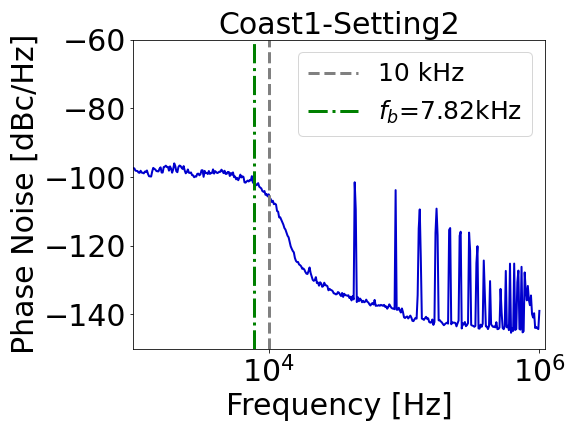
\includegraphics[width=1\textwidth]{images/Ch5/Measured_spectrum_MD5_Coast1-Setting2-PN.csv_no_psd.png}
        %\caption{$y=\sin(2 \pi f t),\ f=50$ Hz}
        %\label{fig:add_label_here}
    \end{subfigure}
    \hfill
    \begin{subfigure}[t]{0.45\textwidth}
        \centering
        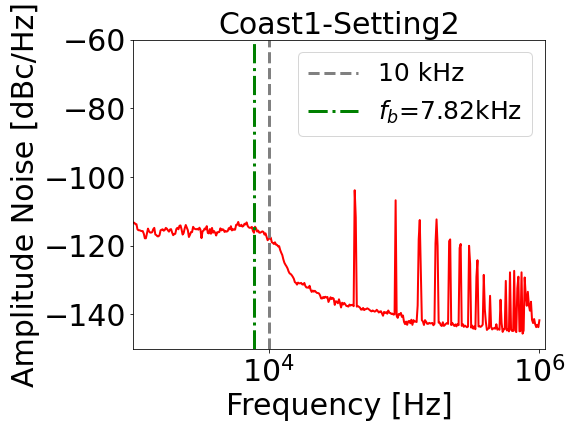
\includegraphics[width=1\textwidth]{images/Ch5/Measured_spectrum_MD5_Coast1-Setting2-AN.csv_no_psd.png}
        %\caption{Discrete Fourier transform}
        %\label{fig:add_label_here}
    \end{subfigure}
    \hfill
     \caption{Example phase (left) and amplitude (right) noise spectra measured with a spectrum analyzer E5052B during the emittance growth studies with CCs in SPS. The noise spread-out up to 10\,kHz (grey dashed line) exciting the first betatron sideband at $\sim$8\,kHz (green dashed line). The spikes seen in the right side of the spectrum appear at multiples of the revolution frequency and are a result of the bunch crossing.} % bunch passage
     \label{fig:example_PN_and_AN}
\end{figure}


 After the examples mention the need for introducing the effective phase noise. (Do I need extra details?)
 

 - effective noise
 - Comparison to the theroeical --> mention further explanation is provided ip 

 \section{Comparison with the theory}\label{sec:MD2018_vs_theory}